\documentclass[UTF8]{ctexart}
\usepackage{amsmath,amssymb}
\usepackage{fancyhdr}
\usepackage{amsmath,bm}
\usepackage{mathrsfs}
\usepackage{ntheorem}
\usepackage{graphicx}
\usepackage{subfigure}
\usepackage[top=2cm, bottom=2cm, left=2cm, right=2cm]{geometry}  
\usepackage{algorithm}  
\usepackage{algorithmicx}  
\usepackage{algpseudocode}
\usepackage{multirow}
\usepackage{tikz}
\usepackage{listings}
\usepackage{xcolor}
\usetikzlibrary{automata, positioning, arrows}
\tikzset{
    ->,
    >=stealth,
    node distance = 3cm,
    every state/.style={thick, fill=gray!10},
    initial text=$ $
}
\lstset{numbers=left, %设置行号位置
        numberstyle=\tiny, %设置行号大小
        keywordstyle=\color{blue}, %设置关键字颜色
        commentstyle=\color[cmyk]{1,0,1,0}, %设置注释颜色
        frame=single, %设置边框格式
        escapeinside=``, %逃逸字符(1左面的键),用于显示中文
        %breaklines, %自动折行
        extendedchars=false, %解决代码跨页时,章节标题,页眉等汉字不显示的问题
        xleftmargin=2em,xrightmargin=2em, aboveskip=1em, %设置边距
        tabsize=4, %设置tab空格数
        showspaces=false %不显示空格
    }
\floatname{algorithm}{算法}  
\renewcommand{\algorithmicrequire}{\textbf{输入:}}  
\renewcommand{\algorithmicensure}{\textbf{输出:}}  

\theorembodyfont{\normalfont\rm\CJKfamily{song}}
%\theoremstyle{break}
\newtheorem{theorem}{定理}
\newtheorem{lemma}{引理}
\newtheorem{proposition}{命题}
\newtheorem*{proof}{证}[section]
\newtheorem*{solution}{解}[section]
\title{运行时存储管理作业}
\author{丁元杰 17231164}
\date{\today}

\begin{document}
\maketitle

\section*{6-1.1}
例子:
\begin{itemize}
    \item 使用函数进行的内存分配请求,例如malloc函数。
    \item 动态类型语言,例如Python和Ruby。
\end{itemize}

\section*{6-2.2}
①时刻的栈参见\ref{1}
\begin{table}[htbp!]
    \centering
    \begin{tabular}{|c|}
        \hline 
        R \\
        \hline
        prevabp \\
        \hline
        ret addr(3) \\
        \hline
        abp(3) \\
        \hline
        S \\
        \hline
        J, X, Y \\
        \hline
        prevabp \\
        \hline
        ret addr(2)\\
        \hline
        abp(2)\\
        \hline
        I, X, Y \\
        \hline
        
    \end{tabular}
    \caption{①时刻的栈}
    \label{1}
\end{table}

②时刻的栈参见\ref{2}:

\begin{table}[htbp!]
    \centering
    \begin{tabular}{|c|}
        \hline
        S \\
        \hline
        J, X, Y \\
        \hline
        prevabp \\
        \hline
        ret addr(2)\\
        \hline
        abp(2)\\
        \hline
        I, X, Y \\
        \hline
    \end{tabular}
    \caption{②时刻的栈}
    \label{2}
\end{table}

\section*{6-2.3}
参见图\ref{stack}
\begin{figure}[htbp!]
    \centering
    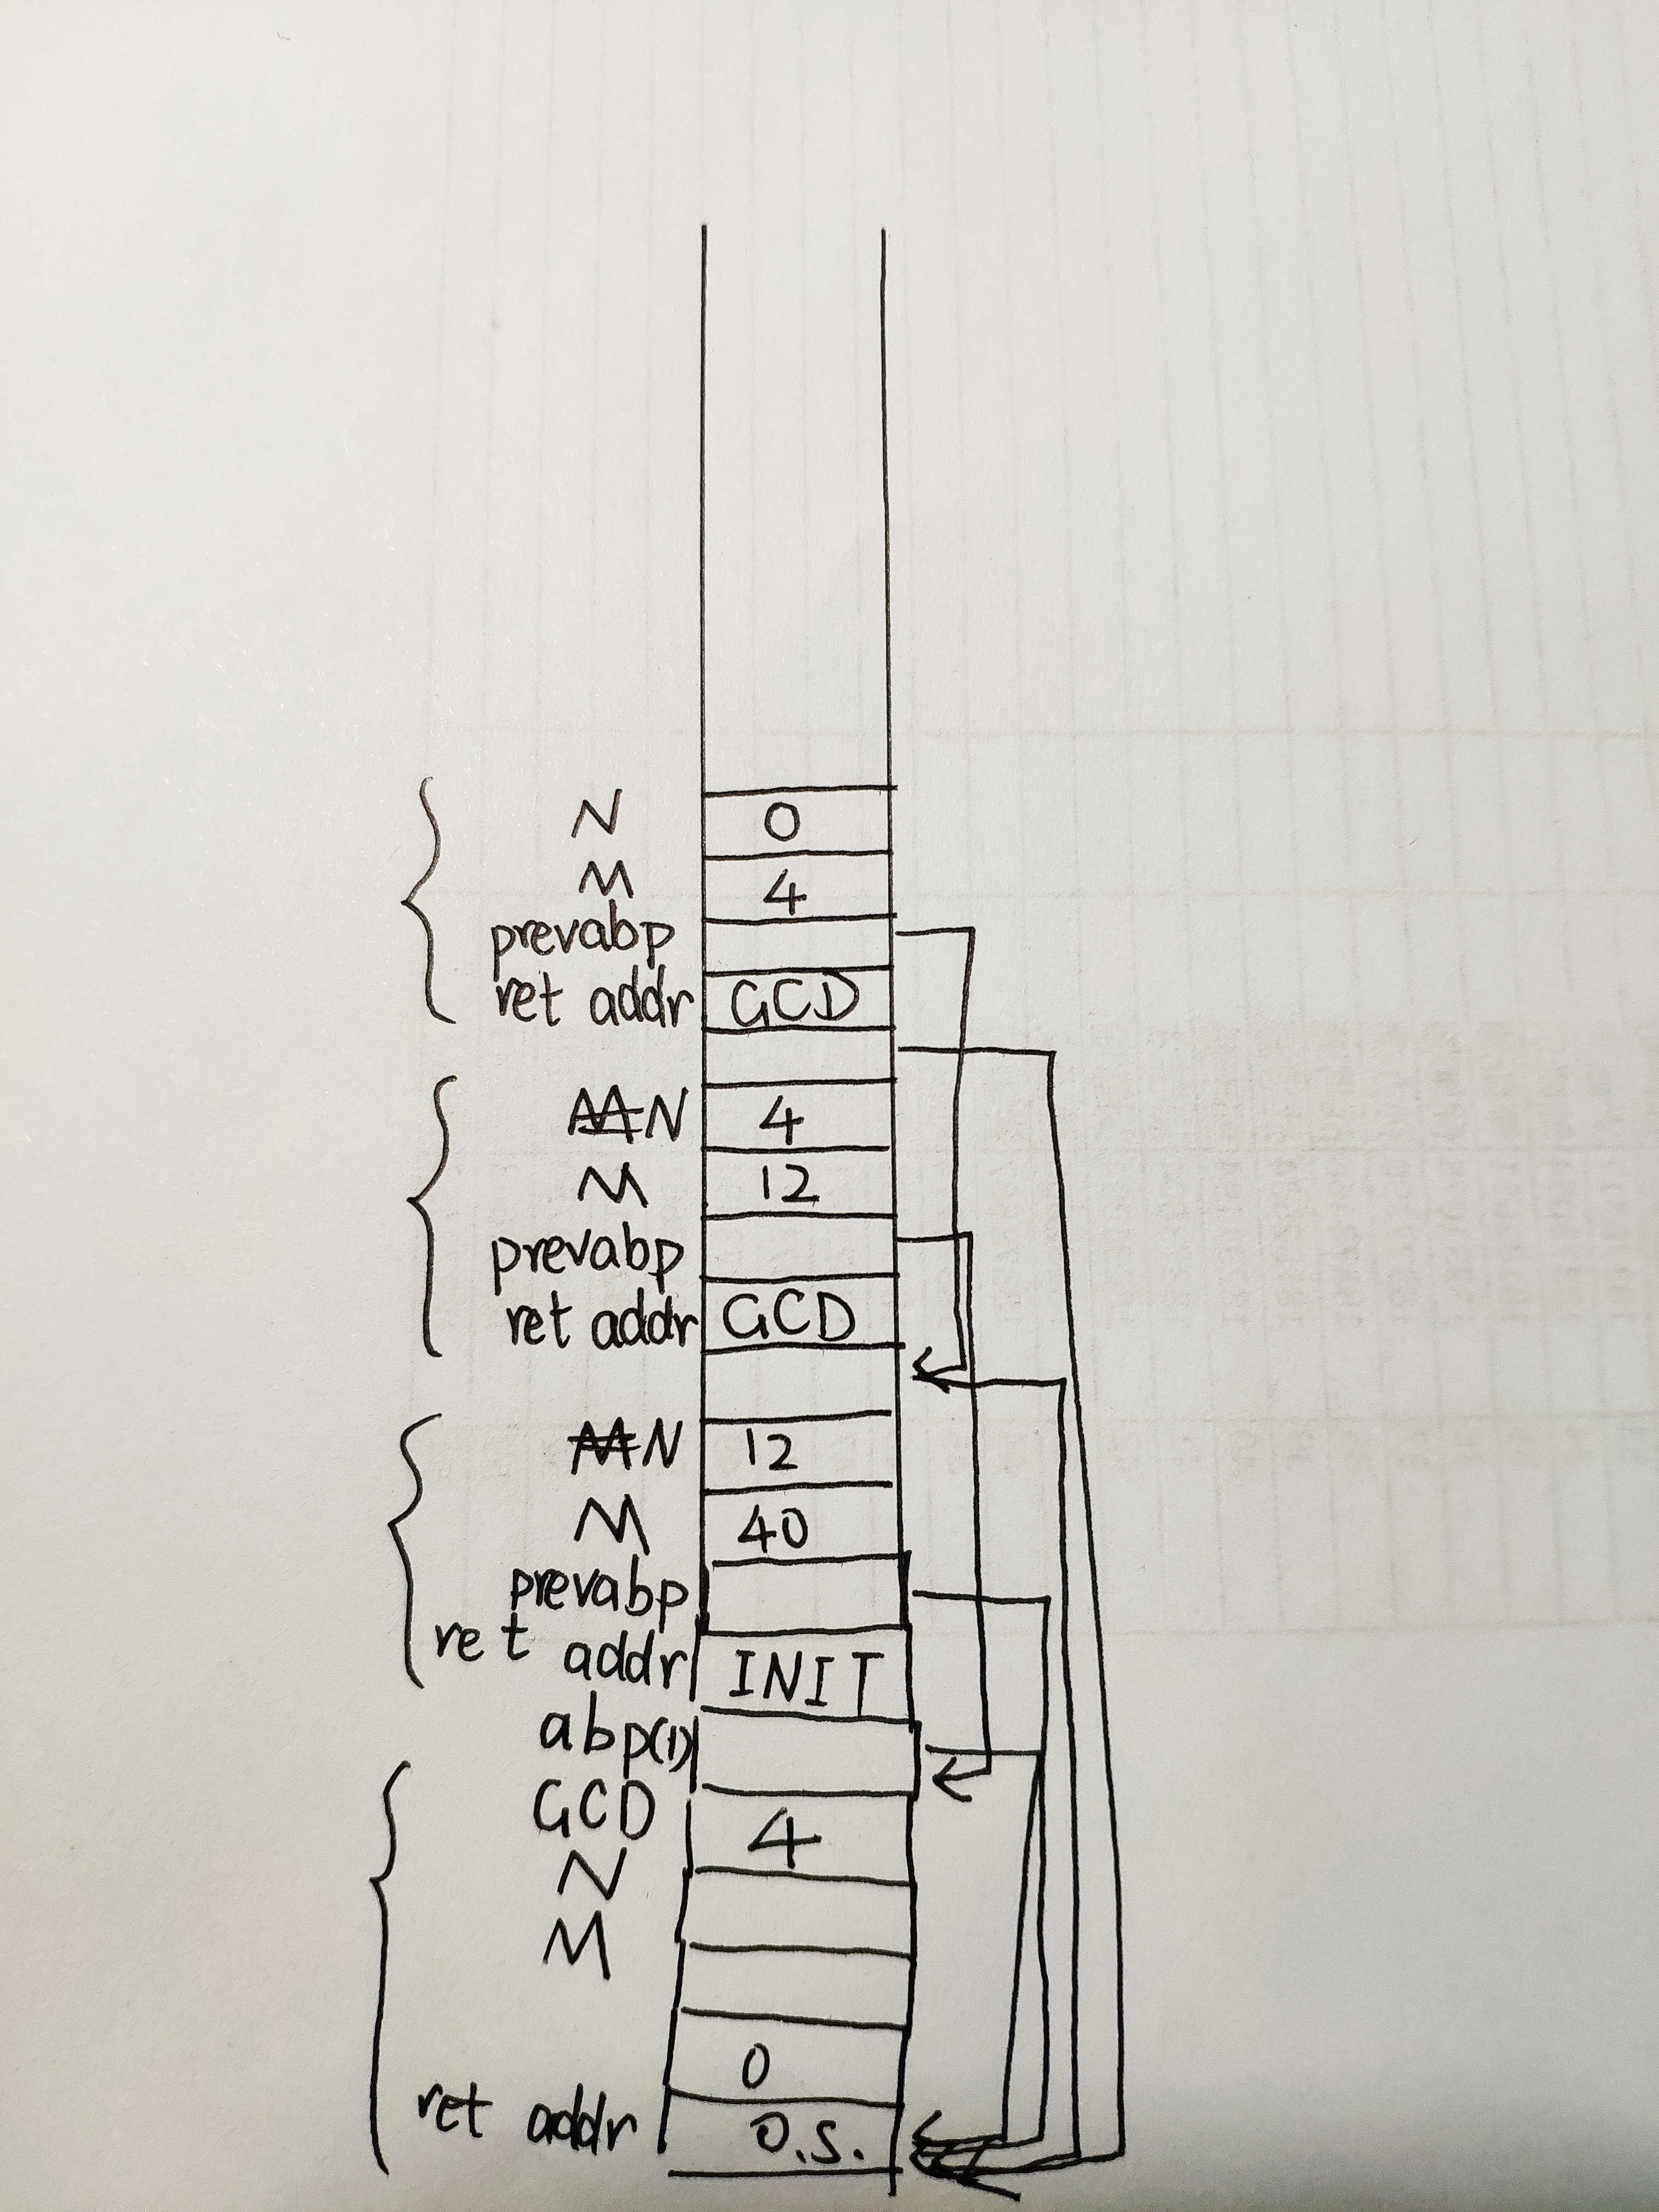
\includegraphics[scale=0.1]{6-2-3.jpg}
    
    \caption{GCD的运行栈}
    \label{stack}
\end{figure}

\end{document}